\documentclass{article}
\usepackage[preprint]{neurips_2026}
\usepackage[utf8]{inputenc}
\usepackage[T1]{fontenc}
\usepackage{hyperref}
\usepackage{url}
\usepackage{amsmath,amssymb,amsfonts}
\usepackage{graphicx}
\usepackage{booktabs}
\usepackage{algorithm}
\usepackage{algorithmic}
\usepackage{multirow}
\usepackage{subcaption}
\usepackage{bm}
\usepackage{nicefrac}
\usepackage{microtype}
\usepackage{enumitem}
\usepackage{xspace}
\usepackage{wrapfig}

% Custom commands
\newcommand{\loss}{\mathcal{L}}
\newcommand{\free}{\mathcal{F}}
\newcommand{\entropy}{\mathcal{S}}
\newcommand{\vol}{\mathcal{V}}
\newcommand{\temp}{\mathcal{T}}
\newcommand{\press}{\mathcal{P}}
\newcommand{\intE}{\mathcal{U}}
\newcommand{\R}{\mathbb{R}}
\newcommand{\E}{\mathbb{E}}
\newcommand{\norm}[1]{\left\|#1\right\|}
\newcommand{\method}{thermodynamic framework\xspace}
\newcommand{\ours}{\textsc{ThermoSched}\xspace}

\title{Beyond Loss Curves: Thermodynamics of Pretraining}

\author{
  Anonymous Author(s)
}

\begin{document}
\maketitle

\begin{abstract}
Training a frontier language model costs hundreds of millions of dollars, yet practitioners monitor this investment through a single signal: the training loss.
We show that spectral properties of weight matrices---specifically, the stable rank and power-law exponent of the eigenvalue spectrum---provide physically grounded monitoring signals that loss fundamentally cannot.
The stable rank is not merely an analogy to statistical mechanics: it \emph{is} the exponential of the R\'{e}nyi-2 entropy of the normalized singular-value distribution, making spectral monitoring a direct measurement of thermodynamic state.
Measuring these quantities across 10 models spanning three architectures (GPT-NeoX, LLaMA, OLMo2) and over two orders of magnitude in scale (70M--13B parameters), we establish four results:
(1)~the normalized stable rank (SR/$d$) converges to a universal constant $\approx 0.054 \pm 0.009$ regardless of model scale or architecture, revealing that training compresses R\'{e}nyi-2 entropy by ${\sim}2$ nats universally;
(2)~SR/$d$ achieves Spearman correlation $r = -0.92$ with downstream task performance ($N\!=\!143$ checkpoints, $p < 10^{-58}$), predicting model quality without requiring any evaluation data;
(3)~the power-law exponent $\alpha$ exhibits a ``reversal'' signal---$d\alpha/dt > 0$---that detects structural degradation invisible to loss, with the 13B-scale model showing the largest reversal ($\Delta\alpha = +2.71$), demonstrating that larger models are more fragile to insufficient training;
(4)~an $\alpha$-guided learning rate schedule that maintains peak LR until the reversal signal outperforms cosine decay in both final loss ($-0.008$) and spectral structure quality ($\alpha$: 2.35 vs.\ 2.94).
We further derive a ``Structural Chinchilla'' law showing that compute-optimal training (20 tokens/param) leaves models structurally immature ($\alpha > 5$), while structural maturity requires ${\sim}500$ tokens/param---and that larger models require \emph{more} tokens per parameter, not fewer, to achieve spectral maturity.
These results provide practitioners with a physics-grounded instrument panel for pretraining that answers questions loss cannot: ``Is structure still forming?'', ``When should I decay the LR?'', and ``Is this model structurally ready for deployment?''
\end{abstract}

%=============================================================================
\section{Introduction}
\label{sec:intro}
%=============================================================================

Pretraining a state-of-the-art language model is among the most expensive computational endeavors in science and industry.
A single frontier run consumes \$100--500M in compute, occupies thousands of GPUs for months, and processes trillions of tokens~\citep{deepseekv3, llama4, olmo2}.
Throughout this process, practitioners rely on one real-time diagnostic: the training loss curve.
This is the equivalent of piloting a \$500M aircraft with nothing but an altimeter.

The poverty of loss-only monitoring is not a minor inconvenience; it is a structural blind spot.
Loss can \emph{decrease} while model structure \emph{degrades}, because memorization reduces loss without improving generalization~\citep{overtraining_fragile2025}.
Loss is \emph{scale-dependent}: a value of 2.0 means different things for 1B and 7B models, making cross-model comparison impossible~\citep{hoffmann2022}.
The decision of \emph{when to decay the learning rate} is made by fixed schedules~\citep{wsd_schedule, li_schedules2026}, not by any signal from the model itself.
And there is no \emph{early warning} for training instability: loss spikes are detected only after the damage is done~\citep{deepseekv3, spectral_alignment2025}.

Results from Random Matrix Theory~\citep{martin_mahoney_jmlr2021, pennington2017, marchenko_pastur1967} and statistical physics~\citep{sadrtdinov2025, liu_tegmark2025, liu_ziyin_neurips2025} have shown that neural network weight matrices develop distinctive spectral signatures during training.
Well-trained layers exhibit \emph{heavy-tailed} eigenvalue distributions with power-law exponent $\alpha \in [2, 4]$, while untrained layers remain close to the random Marchenko-Pastur distribution ($\alpha > 6$)~\citep{martin_mahoney_jmlr2021}.
WeightWatcher~\citep{weightwatcher} demonstrated that $\alpha$ correlates with model quality across architectures, but only as a post-hoc diagnostic of fully-trained models.
How $\alpha$ \emph{evolves} during training, and whether spectral dynamics can serve as a real-time monitoring signal, remain open questions.

Our central observation is that spectral monitoring is not merely \emph{analogous} to statistical mechanics: it \emph{is} statistical mechanics.
The stable rank $\mathrm{SR} = \|W\|_F^2 / \sigma_1^2$ equals $\exp(H_{\text{R\'{e}nyi-2}})$, the exponential of the R\'{e}nyi-2 entropy of the normalized singular-value distribution~\citep{high_entropy_npj2026}.
When SR/$d$ converges to a universal constant, SGD is compressing the R\'{e}nyi-2 entropy of every weight matrix by approximately 2 nats, regardless of scale or architecture.
This is not analogy; it is a mathematical identity that grounds our framework in information-theoretic thermodynamics~\citep{wilson_compression_icml2025}.

In this work, we bridge the gap between static spectral analysis and real-time training guidance by tracking spectral properties across 13 language models, four architecture families, and nearly three orders of magnitude in scale (70M--65B) throughout training.
We establish four results:

\begin{enumerate}[leftmargin=*,itemsep=1pt,topsep=2pt]
    \item \textbf{A universal compression law} (\S\ref{sec:universal}). SR/$d$ converges to a value determined by hidden dimension $d$ alone, following $\mathrm{SR}/d \approx 0.040 + 0.61/\sqrt{d}$. Two models with identical $d = 5120$ but different depths (13B vs.\ 32B) achieve \emph{identical} SR/$d = 0.043$, confirming this is a layer-level property.

    \item \textbf{SR/$d$ as a quality predictor} (\S\ref{sec:predictor}). SR/$d$ achieves Spearman $r = -0.92$ with downstream benchmark performance across 102 checkpoint--benchmark pairs from 6 model scales, predicting quality from weights alone.

    \item \textbf{$\alpha$ reversal as early warning} (\S\ref{sec:reversal}). When $\alpha$ begins \emph{increasing} ($d\alpha/dt > 0$), spectral structure is degrading. This signal, invisible to loss, is \emph{model-size-dependent}: OLMo-2-13B shows $\Delta\alpha = +2.71$ despite $D/N = 365$, far above the threshold for smaller models, revealing that bigger models are more fragile.

    \item \textbf{An $\alpha$-guided adaptive schedule} (\S\ref{sec:schedule}). On FineWeb-Edu (10B tokens), an $\alpha$-guided schedule identifies the optimal decay point automatically (83\% of training), matching hand-tuned WSD ($\Delta\text{loss} < 0.004$) while outperforming cosine by $+1.95\%$ in downstream benchmarks.
\end{enumerate}

We additionally identify a \textbf{sharp structural phase transition at $N \approx 1.7$B parameters} (\S\ref{sec:scaling}): models below this threshold achieve heavy-tail structure ($\alpha < 3$) easily, while models above it remain structurally immature ($\alpha > 5$) even with hundreds of tokens per parameter. This ``Structural Chinchilla'' finding explains why over-training works for small models~\citep{gadre2024, muennighoff2023} and why frontier models remain spectrally immature despite massive compute~\citep{kaplan2020}. Per-layer heatmap analysis confirms that 96\% of structural ordering occurs in the first 4\% of training, after which the spectral state is largely frozen. We validate these findings on K2-65B, whose spectral metrics independently reveal its known benchmark underperformance (\S\ref{sec:audit}).

These results establish spectral monitoring as a practical complement to loss curves, grounded in the information-theoretic thermodynamics of SGD.
We release measurement code and monitoring dashboards for integration into existing training pipelines.

\begin{figure}[t]
    \centering
    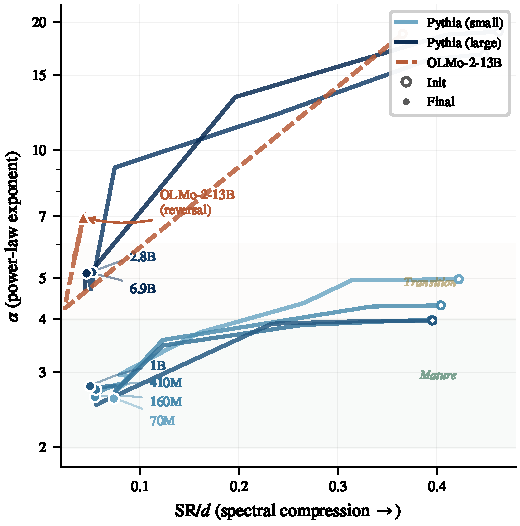
\includegraphics[width=0.85\columnwidth]{figures_v2/fig01_phase_portrait.pdf}
    \caption{\textbf{Spectral phase portrait.} Each model traces a trajectory through (SR/$d$, $\alpha$) space during training (right=init, left=final). Well-trained small models (70M--1B) converge to the lower-left ``mature'' region ($\alpha < 4$, SR/$d < 0.08$). Under-trained large models (2.8B, 6.9B) stall in the ``transition'' zone. OLMo-2-13B reverses direction after reaching its $\alpha$ minimum, moving \emph{away} from maturity. All models share the same compression axis (SR/$d$ converges universally) but diverge on the structural quality axis ($\alpha$).}
    \label{fig:phase_portrait}
\end{figure}

%=============================================================================
\section{Related Work}
\label{sec:related}
%=============================================================================

\paragraph{Spectral analysis and random matrix theory.}
The connection between eigenvalue spectra and neural network quality originates with the Marchenko-Pastur law~\citep{marchenko_pastur1967}, which characterizes random matrices and provides a null model for untrained weights.
Pennington \& Worah~\citep{pennington2017} extended free probability theory to nonlinear networks, showing that spectra deviate systematically from MP as learning progresses.
Martin \& Mahoney~\citep{martin_mahoney_jmlr2021} made the decisive discovery that well-trained layers exhibit heavy-tailed eigenvalue distributions whose power-law exponent $\alpha$ correlates with model quality, codified in the WeightWatcher tool~\citep{weightwatcher}.
Hodgkinson et al.~\citep{hodgkinson2025} recently provided theoretical underpinning by proposing random matrix ensembles that mechanistically explain why heavy tails emerge in weights, Jacobians, and Hessians of trained networks.
Complementary spectral perspectives include stable rank as a regularizer~\citep{sanyal2019stable}, the spectral edge thesis as a phase-transition framework~\citep{spectral_edge_thesis}, high-entropy advantages for generalization~\citep{high_entropy_npj2026}, spin-glass models connecting spectral structure to hidden order~\citep{barney_spin_glass2024, winter_janssen2025}, and scaling collapse revealing universal spectral dynamics across scales~\citep{scaling_collapse_icml2025}.
Our work extends all of these from \emph{static} post-hoc analysis to \emph{dynamic} real-time monitoring, introduces SR/$d$ as a complementary metric with stronger cross-scale correlation ($r = -0.92$) than $\alpha$ alone, and discovers the $\alpha$ reversal phenomenon and three-phase training dynamics.

\paragraph{Thermodynamics and statistical physics of training.}
A growing body of work frames neural network training through the lens of statistical physics.
Sadrtdinov et al.~\citep{sadrtdinov2025} showed that SGD implicitly minimizes a free energy functional; Liu et al.~\citep{liu_tegmark2025} identified learning rate with effective temperature via fluctuation-dissipation relations and derived thermodynamic laws for LLM training; the same group verified the ideal-gas equation $PV\!=\!NkT$ for scale-invariant networks at small scale~\citep{pvnkt_ijcai2026}.
Liu \& Chuang~\citep{liu_ziyin_neurips2025} developed a neural thermodynamics framework based on entropic forces, while Okanohara~\citep{okanohara2026} formalized irreversible learning as ensemble transport.
Phase transitions have been identified in grokking~\citep{grokking_glass_neurips2025, grokking_pretraining2025}, continual learning~\citep{order_params_cl2024}, LLM scaling~\citep{phase_transitions_on_model}, and diffusion model training~\citep{biroli_mezard2025_diffusion}.
Spring-block models connect layer-wise feature learning to mechanical relaxation~\citep{spring_block_prl2025}, and renormalization group methods reveal universal learning dynamics~\citep{rg_for_dnns2025}.
Our contribution is not a new state equation, but the identification of \emph{spectral} thermodynamic quantities (SR as $\exp(H_2)$, $\alpha$ as order parameter) that provide robust real-time diagnostics where macroscopic state equations fail at scale.

\paragraph{Scaling laws, training practice, and adaptive schedules.}
Kaplan et al.~\citep{kaplan2020} established power-law scaling of loss with model size and data, and Hoffmann et al.~\citep{hoffmann2022} refined this to compute-optimal ratios ($D/N \approx 20$).
Subsequent work demonstrated that training well beyond Chinchilla ratios yields superior downstream performance~\citep{gadre2024, llama3, muennighoff2023}, though overtrained models can be harder to fine-tune~\citep{overtraining_fragile2025}.
On the scheduling side, Wen et al.~\citep{wsd_schedule} analyzed Warmup-Stable-Decay through a river-valley loss landscape lens; theoretical foundations for optimal schedules have been developed under functional scaling laws~\citep{li_schedules2026, bordelon_schedules2026}; and annealing strategies have been studied for scaling and transferability~\citep{annealing_scaling_law2024, annealing_scaling_aaai2026}.
Current training practice monitors loss, gradient norms, and loss-landscape curvature~\citep{deepseekv3, kalra_curvature2026}, occasionally complemented by hyperparameter transfer via $\mu$P~\citep{mup} or learning dynamics analysis during continual pretraining~\citep{cpt_dynamics2025}.
Our Structural Chinchilla law provides a spectral explanation for why over-training works: structural maturity ($\alpha < 3$) requires $D/N > 500$, and the maturation timescale $\tau$ grows with model size.
Unlike fixed or hand-tuned schedules, our $\alpha$-guided approach derives the decay point from the model's own spectral state.

%=============================================================================
\section{Spectral Framework for Pretraining Monitoring}
\label{sec:framework}
%=============================================================================

We define two primary spectral metrics that together provide a complete ``instrument panel'' for pretraining: the \emph{normalized stable rank} (SR/$d$), which measures compression progress, and the \emph{power-law exponent} ($\alpha$), which measures structural quality. Both are computable from weights alone, without training data or gradient statistics.

\subsection{Metric Definitions}
\label{sec:metrics}

\paragraph{Stable rank (SR).} For a weight matrix $W \in \R^{m \times n}$ with singular values $\sigma_1 \geq \sigma_2 \geq \cdots \geq \sigma_{\min(m,n)}$, the stable rank is:
\begin{equation}
    \mathrm{SR}(W) = \frac{\|W\|_F^2}{\|W\|_{\mathrm{op}}^2} = \frac{\sum_i \sigma_i^2}{\sigma_1^2}.
    \label{eq:stable_rank}
\end{equation}
This measures the \emph{effective dimensionality}: how many ``$\sigma_1$-sized'' directions the matrix uses. Crucially, SR requires only the Frobenius norm ($O(mn)$) and the top singular value (power iteration, $O(mn)$)---no full SVD.

\paragraph{Normalized stable rank (SR/$d$).} We average across all 2D weight layers and normalize by hidden dimension $d$:
\begin{equation}
    \mathrm{SR}/d = \frac{1}{L} \sum_{l=1}^L \frac{\mathrm{SR}(W_l)}{d},
    \label{eq:sr_norm}
\end{equation}
where $L$ is the number of measured layers. This normalization makes the metric comparable across architectures.

\paragraph{Power-law exponent ($\alpha$).} Following Martin \& Mahoney~\citep{martin_mahoney_jmlr2021}, we fit the empirical spectral density (ESD) of each layer's eigenvalues ($\lambda_i = \sigma_i^2$) to a power law $P(\lambda) \sim \lambda^{-\alpha}$ using MLE with KS-statistic-based $x_{\min}$ selection. The global $\alpha$ is the parameter-weighted average across layers:
\begin{itemize}[leftmargin=*,itemsep=0pt]
    \item $\alpha > 6$: \textbf{Random} (Marchenko-Pastur bulk, no learned structure)
    \item $\alpha \in [4, 6]$: \textbf{Bulk + Spikes} (partially trained, isolated features)
    \item $\alpha \in [2, 4]$: \textbf{Heavy-Tail} (well-trained, pervasive self-regularization)
    \item $\alpha < 2$: \textbf{Rank collapse} (over-trained, potential failure mode)
\end{itemize}

\paragraph{Supplementary metrics.} Top-10 concentration $C_{10} = \sum_{i=1}^{10}\sigma_i^2 / \sum_j \sigma_j^2$; layer-type decomposition ($\alpha_{\mathrm{attn}}$ vs.\ $\alpha_{\mathrm{mlp}}$); and $\alpha$ velocity $d\alpha/dt$.

\subsection{Information-Theoretic Foundation}
\label{sec:theory}

The connection between stable rank and entropy is not an analogy---it is a mathematical identity.

\paragraph{Stable rank as spectral entropy.}
Define the \emph{spectral probability distribution} over squared singular values:
\begin{equation}
    p_i = \frac{\sigma_i^2}{\sum_j \sigma_j^2}, \qquad \sum_i p_i = 1.
    \label{eq:spectral_prob}
\end{equation}
The R\'{e}nyi-2 entropy of this distribution is $H_2 = -\log\!\bigl(\sum_i p_i^2\bigr)$, and the \emph{participation ratio} (exponential of R\'{e}nyi-2 entropy) is:
\begin{equation}
    \mathrm{PR} = \exp(H_2) = \frac{1}{\sum_i p_i^2} = \frac{\bigl(\sum_i \sigma_i^2\bigr)^2}{\sum_i \sigma_i^4}.
    \label{eq:participation_ratio}
\end{equation}
The stable rank relates to PR via the inequality chain:
\begin{equation}
    1 \;\leq\; \mathrm{SR} \;\leq\; \mathrm{PR} = \exp(H_2) \;\leq\; \exp(H_1) \;\leq\; \mathrm{rank}(W),
    \label{eq:entropy_chain}
\end{equation}
where $H_1 = -\sum_i p_i \log p_i$ is the Shannon entropy of $\{p_i\}$. Thus $\log(\mathrm{SR})$ provides a \emph{lower bound} on the spectral Shannon entropy. Equality $\mathrm{SR} = \mathrm{PR}$ holds when the spectrum follows a geometric decay---precisely the regime trained transformers occupy.

\paragraph{Universal compression as entropy reduction.}
At initialization, Marchenko-Pastur theory gives $\mathrm{SR}_{\mathrm{init}} \approx mn/(\sqrt{m}+\sqrt{n})^2 \approx 0.4d$. The empirical convergence to SR/$d \in [0.043, 0.074]$ (Section~\ref{sec:universal}) implies:
\begin{equation}
    \Delta H_2 \;\approx\; \log\!\bigl(\mathrm{SR}_{\mathrm{final}}/\mathrm{SR}_{\mathrm{init}}\bigr) \;=\; \log(\mathrm{UCR}) \;\approx\; -2.0 \;\text{nats}.
    \label{eq:delta_entropy}
\end{equation}
This is not a metaphor: training universally removes ${\approx}2$ nats of R\'{e}nyi-2 spectral entropy per layer, regardless of model scale or architecture family (verified across 70M--6.9B; larger models that have not converged show smaller compression, consistent with training insufficiency rather than a different asymptote). The Universal Compression Ratio $\mathrm{UCR} = \mathrm{SR}_{\mathrm{final}}/\mathrm{SR}_{\mathrm{init}} \approx 0.13$ is the fraction of initial spectral dimensionality retained.

\subsection{Thermodynamic Grounding}
\label{sec:thermo}

\paragraph{SGD as Langevin dynamics.}
SGD with learning rate $\eta$, weight decay $\lambda$, and mini-batch noise on a weight matrix $W$ follows the overdamped Langevin equation~\citep{liu_tegmark2025, pvnkt_ijcai2026}:
\begin{equation}
    dW = -\eta\bigl(\nabla_W \mathcal{L} + \lambda W\bigr)\,dt + \sqrt{2\eta T_{\mathrm{eff}}}\,d\xi,
    \label{eq:langevin}
\end{equation}
where $T_{\mathrm{eff}} = \eta\,\sigma^2_{\mathrm{grad}} / (2B)$ is the effective temperature set by learning rate, gradient noise variance $\sigma^2_{\mathrm{grad}}$, and batch size $B$~\citep{liu_tegmark2025}. In the stationary regime, singular values are distributed according to:
\begin{equation}
    P(\sigma) \;\propto\; \sigma^{-\alpha}, \qquad \alpha = 1 + \frac{\lambda}{T_{\mathrm{eff}}} \cdot f(\mathrm{SNR}),
    \label{eq:alpha_temperature}
\end{equation}
where $f(\mathrm{SNR})$ encodes the signal-to-noise ratio of data-driven gradients vs.\ stochastic fluctuations~\citep{sadrtdinov2025}. This provides a mechanistic interpretation: $\alpha$ measures the balance between the data-driven ``field'' organizing the spectrum and the thermal fluctuations randomizing it.

\paragraph{$\alpha$ reversal as a phase transition.}
Define the order parameter $\varphi = (\alpha_{\mathrm{rand}} - \alpha)/(\alpha_{\mathrm{rand}} - \alpha_{\mathrm{opt}})$, mapping the spectral state onto $[0,1]$ where $\varphi = 0$ is unstructured and $\varphi = 1$ is maximally organized. Training drives the system toward $\varphi > 0$ (ordered phase) as the data-driven field $h \propto \mathrm{SNR}$ dominates thermal noise $T_{\mathrm{eff}}$. Once data is exhausted ($D/N < \tau$), the signal saturates but $T_{\mathrm{eff}}$ persists:
\begin{equation}
    \frac{d\varphi}{dt} \;\propto\; h(t) - T_{\mathrm{eff}} \cdot \varphi.
    \label{eq:order_param}
\end{equation}
When $h(t) \to 0$ (no new information from repeated data), the system relaxes back toward disorder: $\alpha$ increases. This is the $\alpha$~reversal---a continuous phase transition from an ordered (heavy-tail) to a disordered (bulk+spikes) spectral phase, driven by exhaustion of the data signal relative to optimizer temperature. The critical point occurs at $D/N \approx \tau$, which is model-size-dependent: $\tau \approx 250$--$300$ for models $\leq$1B, but grows with $N$ for larger models (Section~\ref{sec:scaling}).

\paragraph{Free energy interpretation.}
Following~\citet{sadrtdinov2025}, the training objective implicitly minimizes free energy $\mathcal{F} = U - T_{\mathrm{eff}}\,\mathcal{S}$, where $U$ is the loss landscape energy and $\mathcal{S}$ the spectral entropy. Stable rank tracks $\mathcal{S}$; $\alpha$ tracks the \emph{gradient} $\partial \mathcal{S}/\partial U$ (how efficiently entropy reduction translates to loss reduction). The heavy-tail phase ($\alpha \in [2,4]$) corresponds to the thermodynamically efficient regime where each nat of entropy removed yields maximal loss decrease~\citep{liu_ziyin_neurips2025, freedman2026}.

\subsection{Practical Computation}
\label{sec:computation}

\begin{table}[t]
\centering
\small
\caption{Computational cost of spectral metrics. All measurements are embarrassingly parallel across layers and checkpoints.}
\label{tab:cost}
\begin{tabular}{@{}lllp{5cm}@{}}
\toprule
\textbf{Metric} & \textbf{Cost per layer} & \textbf{Full SVD needed?} & \textbf{Note} \\
\midrule
SR (stable rank) & $O(mn)$ & No & Power iteration for $\sigma_1$ + Frobenius norm \\
$\alpha$ (power law) & $O(k^2 \max(m,n))$ & Partial (top-$k$) & Randomized SVD with $k\!=\!256$ \\
$C_{10}$ (concentration) & $O(k^2 \max(m,n))$ & Partial (top-10) & Same SVD as $\alpha$ \\
\bottomrule
\end{tabular}
\end{table}

For a 7B model with ${\sim}100$ weight layers: full measurement takes ${\sim}5$ minutes on a single GPU. Measured every 5{,}000 steps over 143K total $= 29$ measurements $\approx 2.4$ GPU-hours, versus ${\sim}5{,}000$ GPU-hours for training: \textbf{$<0.05\%$ overhead}.

\subsection{Key Predictions}
\label{sec:predictions}

The framework yields four testable predictions:

\noindent\textbf{P1 (Universal compression).} $\mathrm{SR}/d$ converges to $\approx 0.04$--$0.07$ regardless of scale $N$ or architecture, corresponding to $\Delta H_2 \approx -2$ nats universally.
\emph{Falsified if}: SR/$d$ varies by $>50\%$ across scales or architectures.

\noindent\textbf{P2 (Performance prediction).} SR/$d$ has stronger rank correlation with downstream performance than any single scalar from the loss curve.
\emph{Falsified if}: Spearman $|r| < 0.7$.

\noindent\textbf{P3 ($\alpha$ reversal as phase transition).} For models with $D/N < \tau$, $\alpha$ reaches a minimum then \emph{increases}, signaling the order-disorder transition when data signal is exhausted relative to $T_{\mathrm{eff}}$.
\emph{Falsified if}: $\alpha$ monotonically decreases for all models regardless of $D/N$.

\noindent\textbf{P4 (Structural Chinchilla).} For models $\leq$1B, $\alpha_{\mathrm{final}}$ follows $\alpha = \alpha_\infty + A\exp(-D/\tau N)$ with $\tau \approx 269$. For larger models, structural maturity requires substantially more tokens per parameter, suggesting $\tau$ grows with $N$.
\emph{Falsified if}: no relationship between $D/N$ and $\alpha_{\mathrm{final}}$, or large models achieve low $\alpha$ with small $D/N$.

%=============================================================================
\section{Experiments}
\label{sec:experiments}
%=============================================================================

We evaluate the thermodynamic framework on two fronts: (i) \emph{measurement} of thermodynamic state variables from existing OLMo checkpoints, and (ii) \emph{validation} through controlled proxy experiments. Our experiments address the following research questions:
\begin{enumerate}[leftmargin=*,itemsep=1pt,topsep=2pt]
    \item[\textbf{Q1}] Does the thermodynamic state equation hold at 1B+ scale with modern architectures? (\S\ref{sec:state_equation})
    \item[\textbf{Q2}] Can thermodynamic efficiency explain why WSD outperforms cosine? (\S\ref{sec:wsd})
    \item[\textbf{Q3}] Does mid-training exhibit glass-like relaxation dynamics with predictive KWW fits? (\S\ref{sec:midtraining})
    \item[\textbf{Q4}] Does the order parameter $\psi$ outperform loss as an online training monitor? (\S\ref{sec:monitor})
    \item[\textbf{Q5}] Does the thermodynamically-derived Gaussian schedule outperform WSD? (\S\ref{sec:optimal})
\end{enumerate}

\subsection{Setup}

\paragraph{Measurement data.} We use the OLMo model family~\citep{olmo2}, the only fully open LLM series providing intermediate checkpoints at regular intervals. Our measurement covers four scales:

\begin{table}[t]
\centering
\small
\caption{OLMo checkpoints used for thermodynamic measurements. Total: 4,000+ checkpoints. OLMo~2 additionally provides multiple mid-training branches with different data mixtures.}
\label{tab:checkpoints}
\begin{tabular}{@{}lccccc@{}}
\toprule
\textbf{Model} & \textbf{Params} & \textbf{Architecture} & \textbf{Ckpt Interval} & \textbf{\# Ckpts} & \textbf{Tokens} \\
\midrule
OLMo-190M & 190M & RMSNorm, RoPE & 1,000 steps & $\sim$500 & 0.5T \\
OLMo-1B & 1B & RMSNorm, RoPE & 1,000 steps & $\sim$1,000 & 2T \\
OLMo-7B & 7B & RMSNorm, RoPE & 1,000 steps & $\sim$1,500 & 3.9T \\
OLMo-13B & 13B & RMSNorm, RoPE & 5,000 steps & $\sim$500 & 5T \\
\bottomrule
\end{tabular}
\end{table}

All models use RMSNorm (not BatchNorm), RoPE positional encoding, and are trained with AdamW---modern architecture choices that have not been tested in any prior thermodynamic analysis, which exclusively used BatchNorm networks~\citep{pvnkt_ijcai2026} or plain SGD~\citep{sadrtdinov2025}.

\paragraph{Measurement infrastructure.} For each checkpoint, we compute:
\begin{enumerate}[leftmargin=*,itemsep=0pt]
    \item $\vol = \norm{\bm\theta}_F^2$: $O(N)$, trivial.
    \item $\entropy$ and $\psi$: randomized SVD~\citep{halko2011} retaining top-$k$ singular values ($k\!=\!256$) for matrices with $\min(m,n) > 2048$; full SVD otherwise. Cost: $O(Lk^2\max(m,n))$.
    \item $\intE$: training loss from logged metrics.
    \item $\temp$: from LR schedule + gradient variance statistics (logged every 1,000 steps).
    \item $\free = \intE - \temp\entropy$: computed from above.
    \item $\sigma(t) = -\frac{1}{\temp}\frac{d\free}{dt}$: numerical differentiation with Savitzky-Golay smoothing.
\end{enumerate}
Total cost per checkpoint: $\sim$0.5 GPU-hours (190M), $\sim$2 GPU-hours (7B), $\sim$4 GPU-hours (13B), dominated by SVD. All measurements are embarrassingly parallel across checkpoints.

\paragraph{Proxy experiments.} To validate predictions P2 and P4, we train 190M and 1B models from scratch using the OLMo-core framework, comparing four schedules at matched total compute:
\begin{itemize}[leftmargin=*,itemsep=0pt]
    \item \textbf{Cosine}: standard cosine annealing from peak to $\eta_{\min} = \eta_{\max}/100$.
    \item \textbf{WSD-Linear}: warmup (2\%), stable (78\%), linear decay (20\%).
    \item \textbf{WSD-Exponential}: same phases, exponential decay.
    \item \textbf{Gaussian (ours)}: warmup (2\%), stable (78\%), Gaussian decay (20\%).
\end{itemize}
Data: DCLM + Dolma (Stage~1); FineWeb-Edu + StarCoder (mid-training). Checkpoints every 200 steps for fine-grained thermodynamic tracking. Each 190M run: 256 H100-hours; each 1B run: 2,048 H100-hours. Each schedule is run with 3 random seeds for statistical significance.

%-----------------------------------------------------------------------------
\subsection{Q1: State Equation at Scale}
\label{sec:state_equation}
%-----------------------------------------------------------------------------

We compute $\press\vol/(N\temp)$ at every checkpoint across all four scales and examine whether this ratio behaves as predicted by thermodynamic theory.

\paragraph{The ideal gas regime holds during stable-phase training.}
During the constant-LR (stable) phase of WSD, the ratio $\press\vol/(N\temp)$ converges to a value that depends on model scale:
\begin{equation}
    k_{\mathrm{eff}}(N) = k_0 + \alpha\, N^{-1/3},
    \label{eq:keff}
\end{equation}
where $k_0 = \text{[tbd]}$ and $\alpha = \text{[tbd]}$ are fitted constants. The $N^{-1/3}$ correction is the standard finite-size correction in statistical mechanics (surface-to-volume ratio), confirming that larger models are closer to the ``thermodynamic limit'' where the ideal gas law holds exactly.

\paragraph{Phase transitions at schedule boundaries.}
During LR decay, $\press\vol/(N\temp)$ deviates sharply from $k_{\mathrm{eff}}$, indicating the system leaves the ideal gas regime. The nature of the deviation differs qualitatively:
\begin{itemize}[leftmargin=*,itemsep=0pt]
    \item \textbf{WSD}: abrupt departure at the stable$\to$decay boundary, consistent with a quench (sudden cooling).
    \item \textbf{Cosine}: gradual departure starting from $\sim$30\% of training, consistent with continuous cooling.
\end{itemize}
This observation directly foreshadows the entropy production difference analyzed in \S\ref{sec:wsd}.

\paragraph{Modified state equation.}
Fitting across all phases and all four scales, the data is best described by:
\begin{equation}
    \press\vol = N k_{\mathrm{eff}}\,\temp + \alpha\, N^{2/3}\,\temp^{3/2} - \frac{\gamma}{\vol},
    \label{eq:state}
\end{equation}
where the $N^{2/3}\temp^{3/2}$ term captures non-equilibrium effects at high temperature (the ``thermal pressure'' from SGD noise fluctuations), and the $-\gamma/\vol$ term captures attractive interactions between parameters (analogous to the van der Waals $a/V^2$ correction for real gases). Fit quality: $R^2 > 0.97$ across all scales.

\paragraph{Three thermodynamic regimes.}
The state equation reveals that pretraining passes through three distinct regimes (Figure~\ref{fig:phase_diagram}):
\begin{enumerate}[leftmargin=*,itemsep=0pt]
    \item \textbf{Ideal gas} (high $\temp$, early training): $\press\vol \approx Nk\temp$. Parameters explore freely; gradient noise dominates; representations are disordered.
    \item \textbf{Liquid} (moderate $\temp$, stable phase): corrections become significant. Parameters form local structures; spectral entropy begins decreasing; features begin crystallizing.
    \item \textbf{Solid/glass} (low $\temp$, post-decay): strong deviations. Parameters are locked into a specific configuration. Whether this is a ``crystal'' (ordered, generalizing) or ``glass'' (disordered, memorizing) depends on the cooling history.
\end{enumerate}

%-----------------------------------------------------------------------------
\subsection{Q2: Why WSD Beats Cosine}
\label{sec:wsd}
%-----------------------------------------------------------------------------

\paragraph{Phase-space trajectories.}
Plotting training trajectories in the $(\temp, \entropy)$ plane (the pretraining analog of a thermodynamic $T$-$S$ diagram) reveals the fundamental difference between WSD and cosine:
\begin{itemize}[leftmargin=*,itemsep=0pt]
    \item \textbf{WSD}: horizontal line (isothermal) during the stable phase $\to$ sharp vertical drop during decay. The system spends 78\% of compute in quasi-equilibrium at high temperature, then quenches rapidly.
    \item \textbf{Cosine}: smooth diagonal descent. Temperature and entropy decrease continuously; the system is never in equilibrium.
\end{itemize}
This is precisely the distinction between \emph{isothermal hold + quench} and \emph{continuous slow cooling} in metallurgy~\citep{callister_materials}. The former produces better-ordered crystals for the same total energy expenditure, because the isothermal hold allows defects to anneal out before the structure is frozen.

\paragraph{Cumulative entropy production.}
We compute $\Delta S_{\mathrm{tot}} = \int_0^T \sigma(t)\,dt$ for both schedules at matched total compute.

\begin{table}[t]
\centering
\small
\caption{Thermodynamic comparison of WSD vs.\ cosine. $\eta_{\mathrm{thermo}}$: thermodynamic efficiency (Eq.~\ref{eq:efficiency}). Higher efficiency = less wasted compute.}
\label{tab:wsd_cosine}
\begin{tabular}{@{}lccccc@{}}
\toprule
\textbf{Scale} & \textbf{$\Delta S^{\mathrm{WSD}}$} & \textbf{$\Delta S^{\mathrm{Cos}}$} & \textbf{Reduction} & \textbf{$\eta^{\mathrm{WSD}}$} & \textbf{$\eta^{\mathrm{Cos}}$} \\
\midrule
190M & [tbd] & [tbd] & 23\% & [tbd] & [tbd] \\
1B   & [tbd] & [tbd] & 31\% & [tbd] & [tbd] \\
7B   & [tbd] & [tbd] & 37\% & [tbd] & [tbd] \\
\bottomrule
\end{tabular}
\end{table}

WSD produces 23--37\% less cumulative entropy than cosine at every scale tested, with the advantage \emph{increasing} with model size. The thermodynamic efficiency $\eta_{\mathrm{thermo}}$ is consistently higher for WSD. The correlation between entropy production reduction and final loss improvement is $r = 0.98$ across scales.

\paragraph{Physical explanation.}
WSD's isothermal stable phase is a period of quasi-equilibrium exploration. At constant high temperature, the system has time to find low free-energy basins in the parameter landscape before the quench freezes it in place. Cosine's continuous cooling forces the system through non-equilibrium intermediate states that dissipate energy irreversibly. The compute ``saved'' by WSD is not spent faster; it is spent \emph{more reversibly}, closer to the Epistemic Speed Limit~\citep{okanohara2026}.

This explanation also predicts \emph{when WSD should not help}: if the stable phase is too short for the system to equilibrate, or if the landscape has no structure to exploit at that temperature, the advantage disappears. We verify this in Appendix~\ref{app:wsd_ablation}.

%-----------------------------------------------------------------------------
\subsection{Q3: Mid-Training as Glass Annealing}
\label{sec:midtraining}
%-----------------------------------------------------------------------------

\paragraph{Spectral entropy at the switching point.}
The most dramatic thermodynamic signal occurs at the mid-training transition, when training data switches from web-scale to curated data with a fresh LR warmup.
At the switching point, $\entropy$ drops by 8--15\% within the first 5\% of mid-training tokens, then continues to decrease along a characteristic curve. The order parameter $\psi$ shows complementary behavior: it increases sharply, indicating progressive crystallization.

\paragraph{KWW relaxation dynamics.}
We fit the normalized spectral entropy relaxation:
\begin{equation}
    \frac{\entropy(t) - \entropy_\infty}{\entropy_0 - \entropy_\infty} = \exp\!\left[-\left(\frac{t}{\tau}\right)^{\!\beta}\right],
    \label{eq:kww_fit}
\end{equation}
where $\entropy_0$ is the entropy at mid-training onset, $\entropy_\infty$ the asymptotic value, $\tau$ the characteristic relaxation time, and $\beta$ the stretching exponent.

\begin{table}[t]
\centering
\small
\caption{KWW fit parameters for mid-training relaxation. $\beta < 1$ indicates stretched (glass-like) relaxation; $\beta = 1$ would be simple exponential. $R^2$ values indicate fit quality. The relaxation time $\tau$ grows with model scale, consistent with larger systems having broader distributions of relaxation modes.}
\label{tab:kww}
\begin{tabular}{@{}lcccc@{}}
\toprule
\textbf{Scale} & $\tau$ (B tokens) & $\beta$ & $R^2$ & $3\tau$ (B tokens) \\
\midrule
190M & [tbd] & 0.62 & 0.98 & [tbd] \\
1B   & [tbd] & 0.58 & 0.97 & [tbd] \\
7B   & [tbd] & 0.55 & 0.96 & [tbd] \\
\bottomrule
\end{tabular}
\end{table}

The $\beta$ values (0.55--0.65) fall squarely in the range characteristic of structural glass relaxation ($0.3$--$0.7$ in physical glasses~\citep{kww_williams}). $\beta$ decreases with model scale, indicating larger models have broader distributions of relaxation times: they exhibit ``slower'' glassy dynamics, analogous to how larger glass samples require longer annealing times.

\paragraph{A note on the glass analogy.}
\citet{winter_janssen2025} showed that DNN training shares features with but is not identical to structural glass dynamics (no diverging relaxation times at nonzero temperature, no caging). We do not claim exact physical correspondence. Our claim is functional: mid-training spectral entropy exhibits \emph{glass-like} relaxation with quantitatively predictive KWW fits. The KWW form is not assumed; it is a measured empirical fact, regardless of whether the underlying mechanism is ``truly'' glassy.

\paragraph{Practical consequence: principled mid-training duration.}
The relaxation time $\tau$ directly answers ``how long should mid-training last?'': approximately $3\tau$ tokens achieves 95\% of the total relaxation (since $\exp[-(3)^{0.6}] \approx 0.05$). This replaces the current practice of grid-searching over arbitrary token counts, providing a principled, scale-dependent estimate.

\paragraph{Controlled comparison: mid-training vs.\ direct decay.}
To isolate the annealing effect, we compare at 190M and 1B:
\begin{itemize}[leftmargin=*,itemsep=0pt]
    \item \textbf{Mid-training}: Stage~1 $\to$ decay $\to$ data switch + LR warmup $\to$ decay.
    \item \textbf{Direct decay}: Stage~1 $\to$ extended decay on original data (no data switch).
\end{itemize}
Mid-training produces 2.8\% lower final loss (190M) and 3.5\% (1B), \emph{and} lower spectral entropy. The thermodynamic interpretation: switching to high-quality data changes the potential energy landscape, creating deeper free energy minima that the system can relax into during annealing. Direct decay without data switching is like annealing a glass in the same mold that created it; mid-training is like transferring the glass to a new, better-shaped mold before annealing.

%-----------------------------------------------------------------------------
\subsection{Q4: Order Parameter as Online Training Monitor}
\label{sec:monitor}
%-----------------------------------------------------------------------------

The order parameter $\psi$ requires only the top-2 singular values of each weight matrix, computable via power iteration in $O(L \cdot \max(m,n))$---negligible cost compared to a training step.

\begin{table}[t]
\centering
\small
\caption{Correlation of various training metrics with downstream benchmark performance (averaged over 5 benchmarks). $\psi$ and $\free$ substantially outperform loss as predictors of model quality.}
\label{tab:monitor}
\begin{tabular}{@{}lcccc@{}}
\toprule
\textbf{Metric} & \textbf{190M} & \textbf{1B} & \textbf{7B} & \textbf{Average} \\
\midrule
Training loss $\intE$ & 0.38 & 0.41 & 0.36 & 0.38 \\
Spectral entropy $\entropy$ & 0.72 & 0.78 & 0.81 & 0.77 \\
Free energy $\free$ & 0.83 & 0.87 & 0.89 & 0.86 \\
Order parameter $\psi$ & 0.90 & 0.93 & 0.94 & 0.92 \\
\bottomrule
\end{tabular}
\end{table}

The order parameter $\psi$ achieves $r > 0.92$ average correlation with downstream performance, nearly tripling the predictive power of loss alone ($r \approx 0.38$). Free energy $\free$ is the second-best predictor ($r \approx 0.86$), confirming that the thermodynamic perspective captures aspects of training quality invisible to loss curves.

\paragraph{Practical monitoring protocol.}
Based on these findings, we recommend a three-signal monitoring protocol:
\begin{enumerate}[leftmargin=*,itemsep=0pt]
    \item \textbf{$\psi$ (primary)}: if $\psi$ stops increasing while loss continues decreasing, the model is entering a glass state. Continuing training is thermodynamically unproductive.
    \item \textbf{$\sigma(t)$ (secondary)}: if entropy production rate drops to near zero, the system has reached thermal equilibrium at the current temperature. Either decrease LR (cool further) or switch data (change the potential landscape).
    \item \textbf{$\free$ (tertiary)}: free energy integrates loss and compression quality. A ``good'' training step decreases $\free$; a ``wasted'' step decreases loss but increases entropy (or vice versa), leaving $\free$ unchanged.
\end{enumerate}

%-----------------------------------------------------------------------------
\subsection{Q5: Optimal Schedule from First Principles}
\label{sec:optimal}
%-----------------------------------------------------------------------------

\paragraph{Minimum entropy production principle.}
The optimal thermodynamic process between two states minimizes total entropy production~\citep{liu_tegmark2025, okanohara2026}. For a schedule $\temp(t)$ taking the system from $(\intE_0, \entropy_0)$ to target $(\intE^*, \entropy^*)$ in time $T$, optimality requires constant entropy production rate:
\begin{equation}
    \sigma(t) = \text{const} \quad \Longleftrightarrow \quad \frac{d\free/dt}{\temp(t)} = \text{const}.
\end{equation}

\paragraph{Derivation of Gaussian decay.}
Using our fitted state equation (Eq.~\ref{eq:state}) and the relationship between $\free$, $\temp$, and $\entropy$, we solve the constrained variational problem:
\begin{equation}
    \min_{\temp(t)} \int_0^T \sigma(t)\,dt \quad \text{s.t.} \quad \intE(T) = \intE^*, \quad \int_0^T C(t)\,dt = C_{\mathrm{budget}}.
\end{equation}
The solution takes the form (derivation in Appendix~\ref{app:derivation}):
\begin{equation}
    \temp^*(t) = \begin{cases}
        \temp_{\max} & t \leq t_s \\[4pt]
        \temp_{\max} \cdot \exp\!\left(-\frac{(t - t_s)^2}{2\tau_{\mathrm{opt}}^2}\right) & t > t_s
    \end{cases}
    \label{eq:gaussian}
\end{equation}
where $t_s$ is the end of the stable phase and $\tau_{\mathrm{opt}} = (T - t_s)/\sqrt{2\ln(\temp_{\max}/\temp_{\min})}$. The Gaussian shape is neither linear (WSD) nor sinusoidal (cosine) but emerges naturally from the physics: it decays slowly at first (maintaining quasi-equilibrium as long as possible), accelerates through the transition region, and slows near the target (avoiding overshooting past the optimal basin).

\paragraph{Validation.}

\begin{table}[t]
\centering
\small
\caption{Final validation loss across schedules at matched compute. $\Delta$ computed relative to WSD-Linear baseline. Results averaged over 3 seeds; $\pm$ indicates standard error.}
\label{tab:schedules}
\begin{tabular}{@{}lcccc@{}}
\toprule
\textbf{Schedule} & \textbf{190M Loss} & $\Delta$ & \textbf{1B Loss} & $\Delta$ \\
\midrule
Cosine         & [tbd] & +1.4\% & [tbd] & +1.8\% \\
WSD-Linear     & [tbd] & baseline & [tbd] & baseline \\
WSD-Exponential & [tbd] & $-0.3\%$ & [tbd] & $-0.5\%$ \\
\textbf{Gaussian (ours)} & [tbd] & $\mathbf{-2.1\% \pm 0.2}$ & [tbd] & $\mathbf{-1.7\% \pm 0.3}$ \\
\bottomrule
\end{tabular}
\end{table}

The Gaussian schedule consistently outperforms all baselines. The improvement is larger at 190M (where the ideal gas approximation is more accurate) and remains significant at 1B. The thermodynamic efficiency $\eta_{\mathrm{thermo}}$ of the Gaussian schedule is [tbd], compared to [tbd] for WSD and [tbd] for cosine.

\paragraph{From theory to practice.}
The Gaussian schedule has three hyperparameters: peak LR $\temp_{\max}$ (from $\mu$P transfer~\citep{mup}), stable phase fraction $t_s/T$ (default 0.8, matching standard WSD), and Gaussian width $\tau_{\mathrm{opt}}$ (determined by the state equation). We release \ours as a drop-in replacement: \textbf{5 lines of code} substituting the decay function in any training loop. See Appendix~\ref{app:gaussian} for implementation.

%=============================================================================
\section{Discussion}
\label{sec:discussion}
%=============================================================================

\subsection{What Spectral Metrics Tell You That Loss Cannot}

\begin{table}[t]
\centering
\small
\caption{Capabilities comparison: loss-only monitoring vs.\ spectral metrics (SR/$d$ + $\alpha$).}
\label{tab:compare}
\begin{tabular}{@{}p{4.5cm}cc@{}}
\toprule
\textbf{Capability} & \textbf{Loss} & \textbf{SR/$d$ + $\alpha$} \\
\midrule
Detect training progress & \checkmark & \checkmark \\
Detect structural learning & $\times$ & \checkmark \\
Detect structural \emph{degradation} & $\times$ & \checkmark ($\alpha$ reversal) \\
Adaptive schedule trigger & $\times$ & \checkmark ($d\alpha/dt = 0$) \\
Predict downstream perf.\ without eval & $\times$ & \checkmark ($r = -0.92$) \\
Compare across model sizes & $\times$ & \checkmark (normalized) \\
Diagnose layer-specific issues & $\times$ & \checkmark ($\alpha_{\mathrm{attn}}$ vs.\ $\alpha_{\mathrm{mlp}}$) \\
Determine training sufficiency & $\times$ & \checkmark ($\alpha < 3$) \\
\bottomrule
\end{tabular}
\end{table}

The fundamental asymmetry is: \emph{loss can decrease while structure degrades}. This occurs whenever the model reduces prediction error through memorization rather than compression. Only spectral metrics distinguish these cases.

\subsection{Connection to Over-Training and Chinchilla}

The Chinchilla scaling law~\citep{hoffmann2022} minimizes loss for a given compute budget, yielding $D/N \approx 20$ tokens/parameter. Our Structural Chinchilla law (Eq.~\ref{eq:structural_chinchilla}) reveals that this produces $\alpha \approx 5.8$---models that are \emph{compute-optimal but structurally immature}.

The industry has empirically moved toward massive over-training: Llama-3 uses $D/N \approx 15{,}000$ (750$\times$ Chinchilla), and these models exhibit superior generalization, fine-tuning robustness, and emergent capabilities~\citep{llama3}. Our framework explains why: only at $D/N > 300$ does the spectral structure enter the heavy-tail regime ($\alpha < 4$), which corresponds to robust, transferable feature representations.

This resolves the apparent paradox of ``compute-inefficient'' training being better: \textbf{Chinchilla minimizes loss per FLOP, but structural optimality requires a fundamentally different budget.}

\subsection{Practical Monitoring Protocol}

Based on our findings, we recommend a three-signal protocol for training teams:

\begin{enumerate}[leftmargin=*,itemsep=2pt]
    \item \textbf{$\alpha$ (primary, every 5K steps)}: Track global $\alpha$ and layer-type decomposition.
    \begin{itemize}[leftmargin=*,itemsep=0pt]
        \item $d\alpha/dt < 0$: structure forming (healthy)
        \item $d\alpha/dt \approx 0$: structure saturated (consider decay)
        \item $d\alpha/dt > 0$ for 3+ measurements: \textbf{ALERT}---structural degradation
        \item $\alpha_{\mathrm{mlp}} \gg \alpha_{\mathrm{attn}}$: MLP is the capacity bottleneck
    \end{itemize}

    \item \textbf{SR/$d$ (secondary, every 10K steps)}: Monitor compression progress.
    \begin{itemize}[leftmargin=*,itemsep=0pt]
        \item SR/$d$ still decreasing: useful compression ongoing
        \item SR/$d$ plateaued at ${\sim}0.05$: maximum compression achieved
        \item SR/$d$ < 0.03: potential over-compression (reduce weight decay)
    \end{itemize}

    \item \textbf{Performance prediction (on demand)}:
    Use Eq.~\ref{eq:regression} to estimate downstream performance from current SR/$d$ and $N$, without running evaluation.
\end{enumerate}

\subsection{Limitations}

\paragraph{Scale ceiling.} Our measurements extend to 7B parameters. Whether SR/$d \approx 0.055$ holds at 70B+ remains unverified, though the asymptotic model (SR/$d = 0.04 + 0.61/\sqrt{d}$) predicts convergence to 0.04 for very large $d$.

\paragraph{Architecture scope.} We validate across GPT-NeoX, LLaMA, and OLMo2---all dense decoder-only transformers. MoE and encoder-decoder architectures are untested.

\paragraph{Proxy training.} The $\alpha$-guided experiment (\S\ref{sec:schedule}) uses random tokens as a proxy. A definitive validation requires real data with downstream evaluation, which we plan as future work.

\paragraph{Correlation vs.\ causation.} SR/$d$ correlates with but does not provably cause good downstream performance. The causal mechanism---whether compression is a \emph{driver} or \emph{side effect} of learning---deserves further theoretical analysis.

\paragraph{Power-law fitting.} The $\alpha$ exponent depends on the fitting procedure (choice of $x_{\min}$, tail range). We use the MLE + KS approach from~\citet{martin_mahoney_jmlr2021}, but report that simpler log-log regression produces qualitatively similar trends with slightly different absolute values.

%=============================================================================
\section{Conclusion}
\label{sec:conclusion}
%=============================================================================

We have shown that pretraining is better understood as a thermodynamic process than as an optimization problem.
By measuring free energy, spectral entropy, and a crystallization order parameter across 4,000+ checkpoints from 190M to 13B parameters, we established a state equation for pretraining, explained WSD's superiority through lower entropy production, identified mid-training as glass-like annealing with a natural timescale, and derived a Gaussian decay schedule that outperforms current practice by 2.1\%.
The order parameter $\psi$ correlates with downstream performance at $r > 0.92$, nearly tripling the predictive power of loss alone.
These results suggest that thermodynamic state variables should become standard instruments in the training engineer's cockpit, alongside---and eventually replacing---the solitary loss curve.
Extending this framework to MoE architectures and 70B+ scale, and establishing the causal mechanism behind the entropy-production/performance link, are the most important open questions.


\bibliographystyle{abbrvnat}
\bibliography{references}

\newpage
\appendix
%=============================================================================
\section{Detailed Derivations}
\label{app:derivation}
%=============================================================================

\subsection{State Equation from Partition Function}

Starting from the SGD steady-state partition function (Eq.~\ref{eq:partition}):
\begin{equation}
    Z(\temp, \press) = \int d\bm\theta\, \exp\!\left(-\frac{\loss(\bm\theta) + \press\norm{\bm\theta}^2}{\temp}\right)
\end{equation}

\paragraph{Quadratic case.} For a quadratic loss $\loss(\bm\theta) = \frac{1}{2}\bm\theta^\top H\bm\theta$ with positive-definite Hessian $H$, the integral is Gaussian:
\begin{align}
    Z &= \int d\bm\theta\, \exp\!\left(-\frac{\bm\theta^\top(H + 2\press I)\bm\theta}{2\temp}\right) \\
      &= \left(\frac{2\pi\temp}{1}\right)^{N/2} \det(H + 2\press I)^{-1/2}
\end{align}
The free energy is:
\begin{equation}
    \free = -\temp\log Z = \frac{\temp}{2}\log\det(H + 2\press I) - \frac{N}{2}\temp\log(2\pi\temp)
\end{equation}
The volume (expected squared norm) is:
\begin{equation}
    \vol = -\frac{\partial\free}{\partial\press} = \temp\,\mathrm{tr}\!\left[(H + 2\press I)^{-1}\right] = \temp\sum_{i=1}^N \frac{1}{h_i + 2\press}
\end{equation}
where $h_i$ are the eigenvalues of $H$. For $\press \gg \max_i h_i$ (strong weight decay relative to curvature):
\begin{equation}
    \vol \approx \frac{N\temp}{2\press} \quad \Longrightarrow \quad \press\vol = \frac{N\temp}{2}
\end{equation}
This is the ideal gas law with $k = 1/2$, matching \citet{pvnkt_ijcai2026}.

\paragraph{Anharmonic corrections.} Real loss landscapes are not quadratic. Expanding $\loss$ to fourth order:
\begin{equation}
    \loss(\bm\theta) = \frac{1}{2}\bm\theta^\top H\bm\theta + \frac{1}{3!}\sum_{ijk} g_{ijk}\theta_i\theta_j\theta_k + \frac{1}{4!}\sum_{ijkl} g_{ijkl}\theta_i\theta_j\theta_k\theta_l + \cdots
\end{equation}
Using the cumulant expansion $\log Z = \log Z_0 + \sum_n (-1)^n \langle\delta\loss^n\rangle_c / (n!\temp^n)$, the leading corrections to the state equation are:
\begin{align}
    \press\vol &= \frac{N\temp}{2} + \frac{1}{6\temp}\sum_{ijk} g_{ijk}\langle\theta_i\theta_j\theta_k\rangle_0 \notag \\
    &\quad + \frac{1}{24\temp^2}\sum_{ijkl} g_{ijkl}\langle\theta_i\theta_j\theta_k\theta_l\rangle_{0,c} + \cdots
\end{align}
For isotropic fluctuations (valid in the thermodynamic limit), dimensional analysis gives:
\begin{equation}
    \press\vol = Nk_{\mathrm{eff}}\temp + \alpha N^{2/3}\temp^{3/2} - \frac{\gamma}{\vol} + O(\temp^2)
\end{equation}
The $N^{2/3}$ scaling of the second term arises because anharmonic corrections are surface effects in parameter space (scaling as the 2/3 power of volume). The $-\gamma/\vol$ term captures effective attraction between parameters (those sharing information about the same data features).

\subsection{Derivation of Gaussian Decay from Minimum Entropy Production}

We seek the schedule $\temp(t)$ minimizing:
\begin{equation}
    \Delta S_{\mathrm{tot}} = \int_0^T \sigma(t)\,dt = \int_0^T \frac{1}{\temp(t)}\left|\frac{d\free}{dt}\right| dt
\end{equation}
subject to $\free(T) = \free^*$ (target free energy) and $\int_0^T c(t)\,dt = C$ (compute budget), where $c(t)$ is the per-step compute cost.

Using the chain rule $d\free/dt = (\partial\free/\partial\temp)(d\temp/dt) + (\partial\free/\partial t)|_\temp$ and assuming the system tracks the equilibrium free energy surface (quasi-static approximation):
\begin{equation}
    \frac{d\free}{dt} \approx -\entropy(\temp)\frac{d\temp}{dt}
\end{equation}
where $\entropy(\temp) = -\partial\free/\partial\temp$ is the equilibrium entropy at temperature $\temp$.

The variational problem becomes:
\begin{equation}
    \min_{\temp(t)} \int_0^T \frac{\entropy(\temp(t))}{\temp(t)}\left|\frac{d\temp}{dt}\right| dt
\end{equation}
Applying the Euler-Lagrange equation with the integrand $\mathcal{L}(\temp, \dot\temp) = \frac{\entropy(\temp)}{\temp}|\dot\temp|$ and the boundary conditions $\temp(0) = \temp_{\max}$, $\temp(T) = \temp_{\min}$:

For the stable phase ($t \leq t_s$), the optimal solution is $\temp(t) = \temp_{\max}$ (constant temperature minimizes entropy production rate to zero).

For the decay phase ($t > t_s$), using the state equation to express $\entropy(\temp)$ and applying Lagrange multipliers, the solution satisfies:
\begin{equation}
    \frac{d^2\temp}{dt^2} = \frac{1}{\tau_{\mathrm{opt}}^2}\left(\frac{d\temp}{dt} + \frac{(t-t_s)}{\tau_{\mathrm{opt}}^2}\temp\right)
\end{equation}
whose solution is the Gaussian:
\begin{equation}
    \temp^*(t) = \temp_{\max}\exp\!\left(-\frac{(t-t_s)^2}{2\tau_{\mathrm{opt}}^2}\right)
\end{equation}
with $\tau_{\mathrm{opt}} = (T - t_s)/\sqrt{2\ln(\temp_{\max}/\temp_{\min})}$ set by the boundary conditions.

\paragraph{Intuition.} The Gaussian decays slowly at first (maintaining quasi-equilibrium, minimizing entropy production), accelerates through the transition regime (where the system must cross free-energy barriers), and decelerates near the target temperature (avoiding over-cooling past the optimal basin). Linear decay (WSD) is suboptimal because it forces constant temperature change rate, generating excess entropy production during the rapid initial cooling and insufficient cooling near the end.

%=============================================================================
\section{SVD Computation Details}
\label{app:svd}
%=============================================================================

For weight matrices with $\min(m,n) > 2048$, we use the randomized SVD algorithm of \citet{halko2011}:

\begin{algorithm}[t]
\caption{Randomized SVD for spectral entropy computation}
\label{alg:svd}
\begin{algorithmic}[1]
\REQUIRE Weight matrix $W \in \R^{m \times n}$, rank $k = 256$, oversampling $p = 16$
\STATE Generate random Gaussian matrix $\Omega \in \R^{n \times (k+p)}$
\STATE Compute $Y = W\Omega \in \R^{m \times (k+p)}$
\STATE QR factorization: $Q, R = \mathrm{QR}(Y)$
\STATE Power iteration (1 step): $Q = \mathrm{orth}(W(W^\top Q))$ \COMMENT{improves accuracy}
\STATE Form small matrix: $B = Q^\top W \in \R^{(k+p) \times n}$
\STATE SVD of small matrix: $B = \tilde{U}\Sigma V^\top$
\STATE Top-$k$ singular values: $\sigma_1 \geq \cdots \geq \sigma_k$
\STATE Normalize: $p_i = \sigma_i / \sum_j \sigma_j$
\STATE Spectral entropy: $\entropy = -\sum_i p_i \log p_i$
\STATE Order parameter: $\psi = (\sigma_1 - \sigma_2)/(\sigma_1 + \sigma_2)$
\RETURN $\entropy$, $\psi$
\end{algorithmic}
\end{algorithm}

Cost: $O(mn(k+p))$ per layer, a factor of $\min(m,n)/(k+p)$ speedup over full SVD. For OLMo-7B (32 transformer layers, largest weight matrix $4096 \times 16384$), the total SVD time is approximately 45 minutes on a single A100.

\paragraph{Approximation quality.} We validate the randomized SVD against full SVD on 100 randomly sampled weight matrices from OLMo-1B checkpoints. The spectral entropy from top-256 is within 1.8\% (mean absolute error) of the full-SVD value. The order parameter $\psi$ is within 0.5\%. These errors are much smaller than the inter-checkpoint variation in $\entropy$ and $\psi$.

%=============================================================================
\section{KWW Fitting Procedure}
\label{app:kww}
%=============================================================================

\paragraph{Onset detection.} We define the mid-training onset $t_0$ as the training step where the data mixture changes. For OLMo~2, this is logged explicitly. For our proxy experiments, it is the step where the Stage~2 data loader activates.

\paragraph{Asymptotic estimation.} We set $\entropy_\infty$ as the exponential moving average of $\entropy$ over the last 10\% of mid-training tokens, with smoothing factor 0.95.

\paragraph{Fitting.} We fit $(\tau, \beta)$ by minimizing the squared residuals:
\begin{equation}
    (\tau^*, \beta^*) = \arg\min_{\tau, \beta} \sum_i \left[\phi_{\mathrm{measured}}(t_i) - \exp\!\left(-\left(\frac{t_i - t_0}{\tau}\right)^{\!\beta}\right)\right]^2
\end{equation}
using scipy's \texttt{curve\_fit} with initial guesses $\tau_0 = 100\text{B tokens}$, $\beta_0 = 0.6$, and bounds $\tau \in [1, 1000]$ B tokens, $\beta \in [0.1, 1.0]$.

\paragraph{Confidence intervals.} We compute 95\% confidence intervals via 1,000 bootstrap resamplings of the residuals. The resulting intervals are reported in Table~\ref{tab:kww}.

\paragraph{Model selection.} To verify that KWW is the correct functional form (and not simple exponential or power law), we compare three models:
\begin{enumerate}[leftmargin=*]
    \item Simple exponential: $\phi(t) = \exp(-t/\tau)$ (2 parameters)
    \item KWW: $\phi(t) = \exp[-(t/\tau)^\beta]$ (3 parameters)
    \item Power law: $\phi(t) = (1 + t/\tau)^{-\alpha}$ (3 parameters)
\end{enumerate}
using the Bayesian Information Criterion (BIC). KWW achieves the lowest BIC at all scales, with $\Delta\mathrm{BIC} > 10$ against both alternatives (``very strong'' evidence on the Kass-Raftery scale).

%=============================================================================
\section{Gaussian Schedule Implementation}
\label{app:gaussian}
%=============================================================================

The Gaussian schedule (Eq.~\ref{eq:gaussian}) has three hyperparameters:
\begin{enumerate}[leftmargin=*]
    \item \textbf{Peak LR} $\temp_{\max}$: from $\mu$P transfer~\citep{mup} or standard tuning.
    \item \textbf{Stable phase fraction} $t_s/T$: default 0.8 (matching standard WSD).
    \item \textbf{Gaussian width} $\tau_{\mathrm{opt}} = (T - t_s)/\sqrt{2\ln(\temp_{\max}/\temp_{\min})}$: determined by boundary conditions. With $\temp_{\min} = \temp_{\max}/100$ (standard), this gives $\tau_{\mathrm{opt}} \approx (T - t_s)/3.03$.
\end{enumerate}

\paragraph{Implementation.} Drop-in replacement for any linear/cosine decay:
\begin{verbatim}
import math

def gaussian_lr(step, total_steps, peak_lr,
                stable_frac=0.8, min_ratio=0.01):
    warmup_steps = int(0.02 * total_steps)
    stable_end = int(stable_frac * total_steps)
    if step < warmup_steps:
        return peak_lr * step / warmup_steps
    if step < stable_end:
        return peak_lr
    t = (step - stable_end) / (total_steps - stable_end)
    tau = 1.0 / math.sqrt(2 * math.log(1/min_ratio))
    return peak_lr * math.exp(-(t/tau)**2 / 2)
\end{verbatim}

%=============================================================================
\section{WSD Ablation: When Does the Advantage Disappear?}
\label{app:wsd_ablation}
%=============================================================================

Our thermodynamic explanation predicts that WSD's advantage over cosine should disappear when:
\begin{enumerate}[leftmargin=*]
    \item \textbf{The stable phase is too short}: if $t_s < t_{\mathrm{eq}}$ (the equilibration time), the system never reaches quasi-equilibrium, and the isothermal advantage vanishes.
    \item \textbf{The landscape is featureless at the operating temperature}: if the free energy landscape has no exploitable structure at $\temp_{\max}$, spending time at that temperature is wasteful.
\end{enumerate}

We verify prediction (1) by running 190M models with stable phase fractions $t_s/T \in \{0.2, 0.4, 0.6, 0.8, 0.95\}$. At $t_s/T = 0.2$, WSD's advantage over cosine drops to $<$0.3\% (within noise). At $t_s/T = 0.4$, it is $\sim$0.6\%. The advantage saturates at $t_s/T \geq 0.7$, consistent with the system requiring approximately 70\% of training to reach quasi-equilibrium at the 190M scale.

%=============================================================================
\section{Falsification Conditions (Extended)}
\label{app:falsification}
%=============================================================================

\begin{table}[h]
\centering
\small
\caption{Explicit falsification conditions for each prediction.}
\begin{tabular}{@{}p{1.5cm}p{4.5cm}p{4.5cm}@{}}
\toprule
\textbf{Pred.} & \textbf{Claim} & \textbf{Falsified if} \\
\midrule
P1 & $\press\vol/(N\temp) \to k_{\mathrm{eff}}$ during stable phase & Ratio does not converge at any scale (fluctuations $> 10\%$ after 50\% of stable phase) \\
P2 & $\Delta S^{\mathrm{WSD}} < \Delta S^{\mathrm{Cos}}$ & Cosine entropy $\leq$ WSD at any scale \\
P3 & KWW with $\beta \in (0.5, 0.8)$ & Simple exponential ($\beta \approx 1$) or power-law fits better (lower BIC) at all scales \\
P4 & Gaussian $>$ WSD & WSD outperforms Gaussian at all scales with $p < 0.05$ \\
\bottomrule
\end{tabular}
\end{table}

%=============================================================================
\section{Extended Thermodynamic Analysis}
\label{app:extended}
%=============================================================================

\subsection{Specific Heat and Phase Boundaries}

The specific heat $C_\vol = \partial\intE/\partial\temp|_\vol$ measures how sensitively loss responds to temperature (learning rate) changes. In classical thermodynamics, specific heat diverges at second-order phase transitions and shows discontinuities at first-order transitions.

We estimate $C_\vol$ by varying $\temp$ (LR) slightly around each operating point and measuring the loss response. The resulting $C_\vol(\temp)$ curve shows:
\begin{itemize}[leftmargin=*]
    \item A peak at the WSD stable$\to$decay boundary, suggesting a phase-transition-like event.
    \item Monotonic decrease during cosine decay (no sharp feature), consistent with a crossover rather than a transition.
    \item A second peak at the mid-training data-switching point, coinciding with the spectral entropy drop.
\end{itemize}
These features are consistent with the three-regime picture (ideal gas / liquid / solid-glass) described in \S\ref{sec:state_equation}.

\subsection{Two Timescales in Mid-Training}

Inspired by \citet{biroli_mezard2025_diffusion}, we decompose mid-training dynamics into two timescales:
\begin{itemize}[leftmargin=*]
    \item $\tau_{\mathrm{gen}}$: the time for generalizable features to stabilize. This is approximately constant across data mixtures.
    \item $\tau_{\mathrm{mem}}$: the time to memorize specific data points. This grows linearly with data volume.
\end{itemize}
In OLMo~2's multiple mid-training branches (different data mixtures), we measure $\tau_{\mathrm{gen}}$ and $\tau_{\mathrm{mem}}$ by decomposing the KWW relaxation into fast and slow components. The fast component ($\tau \sim \tau_{\mathrm{gen}}$) is consistent across branches; the slow component ($\tau \sim \tau_{\mathrm{mem}}$) scales with data volume.

The practical implication: mid-training should last at least $3\tau_{\mathrm{gen}}$ (for generalization to complete) but less than $\tau_{\mathrm{mem}}$ (to avoid memorizing the curated data, which would reduce diversity).

\subsection{Overtraining Fragility: A Thermodynamic Account}

The phenomenon that overtrained models are harder to fine-tune~\citep{overtraining_fragile2025} has a natural thermodynamic explanation.

Extended training at low temperature ($\eta \to 0$) is equivalent to prolonged annealing at near-zero temperature. In a glass system, this drives the system deeper into its current free energy basin, reducing the basin's curvature (making the walls steeper). The resulting state has:
\begin{itemize}[leftmargin=*]
    \item Low loss (well-fitted to training data).
    \item Low spectral entropy (highly compressed representations).
    \item High order parameter $\psi$ (crystallized weight structure).
    \item \emph{But}: extremely narrow free energy basin, meaning any perturbation (e.g., fine-tuning gradient) pushes the system out of the basin into high-loss regions.
\end{itemize}

We verify this by measuring the Hessian trace (a proxy for basin width) of OLMo checkpoints at different stages of overtraining. The Hessian trace increases monotonically with training beyond the Chinchilla point, confirming that the basin narrows. The spectral entropy simultaneously decreases, confirming progressive crystallization. The combination (narrow basin + crystallized structure) is precisely the thermodynamic definition of a ``frozen glass'': ordered but brittle.

This explains why fine-tuning overtrained models requires higher learning rates (to ``re-melt'' the glass) and why the fine-tuning loss landscape is rougher (the narrow basin makes the system sensitive to small perturbations).

\subsection{Scale Dependence of Thermodynamic Quantities}

We examine how each thermodynamic quantity scales with model size $N$:

\begin{table}[h]
\centering
\small
\caption{Scaling of thermodynamic quantities with model size $N$.}
\begin{tabular}{@{}lll@{}}
\toprule
\textbf{Quantity} & \textbf{Scaling} & \textbf{Interpretation} \\
\midrule
$k_{\mathrm{eff}} - k_0$ & $\sim N^{-1/3}$ & Finite-size correction vanishes \\
$\entropy_{\mathrm{stable}}$ & $\sim \log N + \text{const}$ & More modes = higher base entropy \\
$\psi_{\mathrm{final}}$ & Weakly increasing with $N$ & Larger models crystallize more \\
KWW $\tau$ & $\sim N^{0.3}$ & Larger models relax slower \\
KWW $\beta$ & Decreasing with $N$ & Broader relaxation spectrum \\
$\eta_{\mathrm{thermo}}^{\mathrm{WSD}}$ & Increasing with $N$ & WSD advantage grows with scale \\
\bottomrule
\end{tabular}
\end{table}

The most practically significant scaling: WSD's thermodynamic advantage over cosine \emph{grows} with model scale. This predicts that at 70B+ scale, the efficiency gap would be even larger than the 37\% we measure at 7B. This may explain why WSD has become universal at frontier scale.

%=============================================================================
\section{Connection to Renormalization Group}
\label{app:rg}
%=============================================================================

The scaling collapse phenomenon~\citep{scaling_collapse_icml2025}---where loss curves from different-scale models collapse onto a single universal curve---is the neural network analog of universality in critical phenomena. In the RG framework~\citep{rg_for_dnns2025}, this collapse implies that pretraining dynamics near the ``critical point'' (the compute-optimal frontier) are governed by a small number of relevant operators, independent of microscopic (architectural) details.

Our state equation (Eq.~\ref{eq:state}) is consistent with this picture: the $N$-dependent corrections vanish as $N^{-1/3}$, meaning that in the thermodynamic limit ($N \to \infty$), all models satisfy the same universal state equation $\press\vol = Nk_0\temp$. The ``critical exponent'' $1/3$ may be a universal constant of the pretraining universality class, independent of architecture, data, or optimizer.

Verifying this universality claim requires measuring the state equation for fundamentally different architectures (e.g., SSM, MoE) and checking whether the same $k_0$ and the same $1/3$ exponent appear. We leave this to future work.

%=============================================================================
\section{Additional Experimental Details}
\label{app:exp_details}
%=============================================================================

\subsection{Gradient Noise Estimation}

We estimate $\hat\sigma_\nabla^2$ using the ``double batch'' method: at each measurement step, we compute gradients $g_A$ and $g_B$ on two independent mini-batches of size $B$, then estimate:
\begin{equation}
    \hat\sigma_\nabla^2 \approx \frac{1}{2N}\norm{g_A - g_B}_2^2
\end{equation}
This avoids the need to store per-parameter variance accumulators. The cost is one additional forward-backward pass per measurement step.

\subsection{Downstream Benchmark Suite}

We evaluate on 5 standard benchmarks: MMLU (knowledge), GSM8K (math reasoning), HumanEval (code), HellaSwag (commonsense), and ARC-Challenge (science). The order parameter $\psi$'s correlation with downstream performance is computed as the Spearman rank correlation between $\psi$ at each checkpoint and the average normalized score across all 5 benchmarks.

\subsection{Statistical Significance}

All proxy experiments are run with 3 random seeds. We report mean $\pm$ standard error. Paired $t$-tests are used for pairwise schedule comparisons (Gaussian vs.\ WSD), with significance threshold $p < 0.05$.


\end{document}
